% !TEX root = ../YourName-Dissertation.tex

\chapter{Direct Measurement of the Neutrino Mass with Cyclotron Radiation Emission Spectroscopy}

\section{Introduction}

\section{Cyclotron Radiation Emission Spectroscopy}

Of the standard physical quantities the one that can be measured with the highest precision is time and the inversely related quantity frequency. In fact it is often advantageous to convert measurements of other physical quantities like mass or length into frequency measurements due to the digital nature of frequency measurements that make them immune to many sources of noise. Atomic clocks, which operate by measuring the frequencies of various atomic transitions, have been used to measure time with astounding relative uncertainties of $10^{-18}$~seconds. The extreme precision possible with frequency measurements is often summarized using the a quote from the Physicist Arthur Schawlow who said advise his students to "Never measure anything but frequency!". 

Neutrino mass measurements using tritium beta-decay are effectively attempting to measure  

\begin{figure}[htbp]
    \centering
    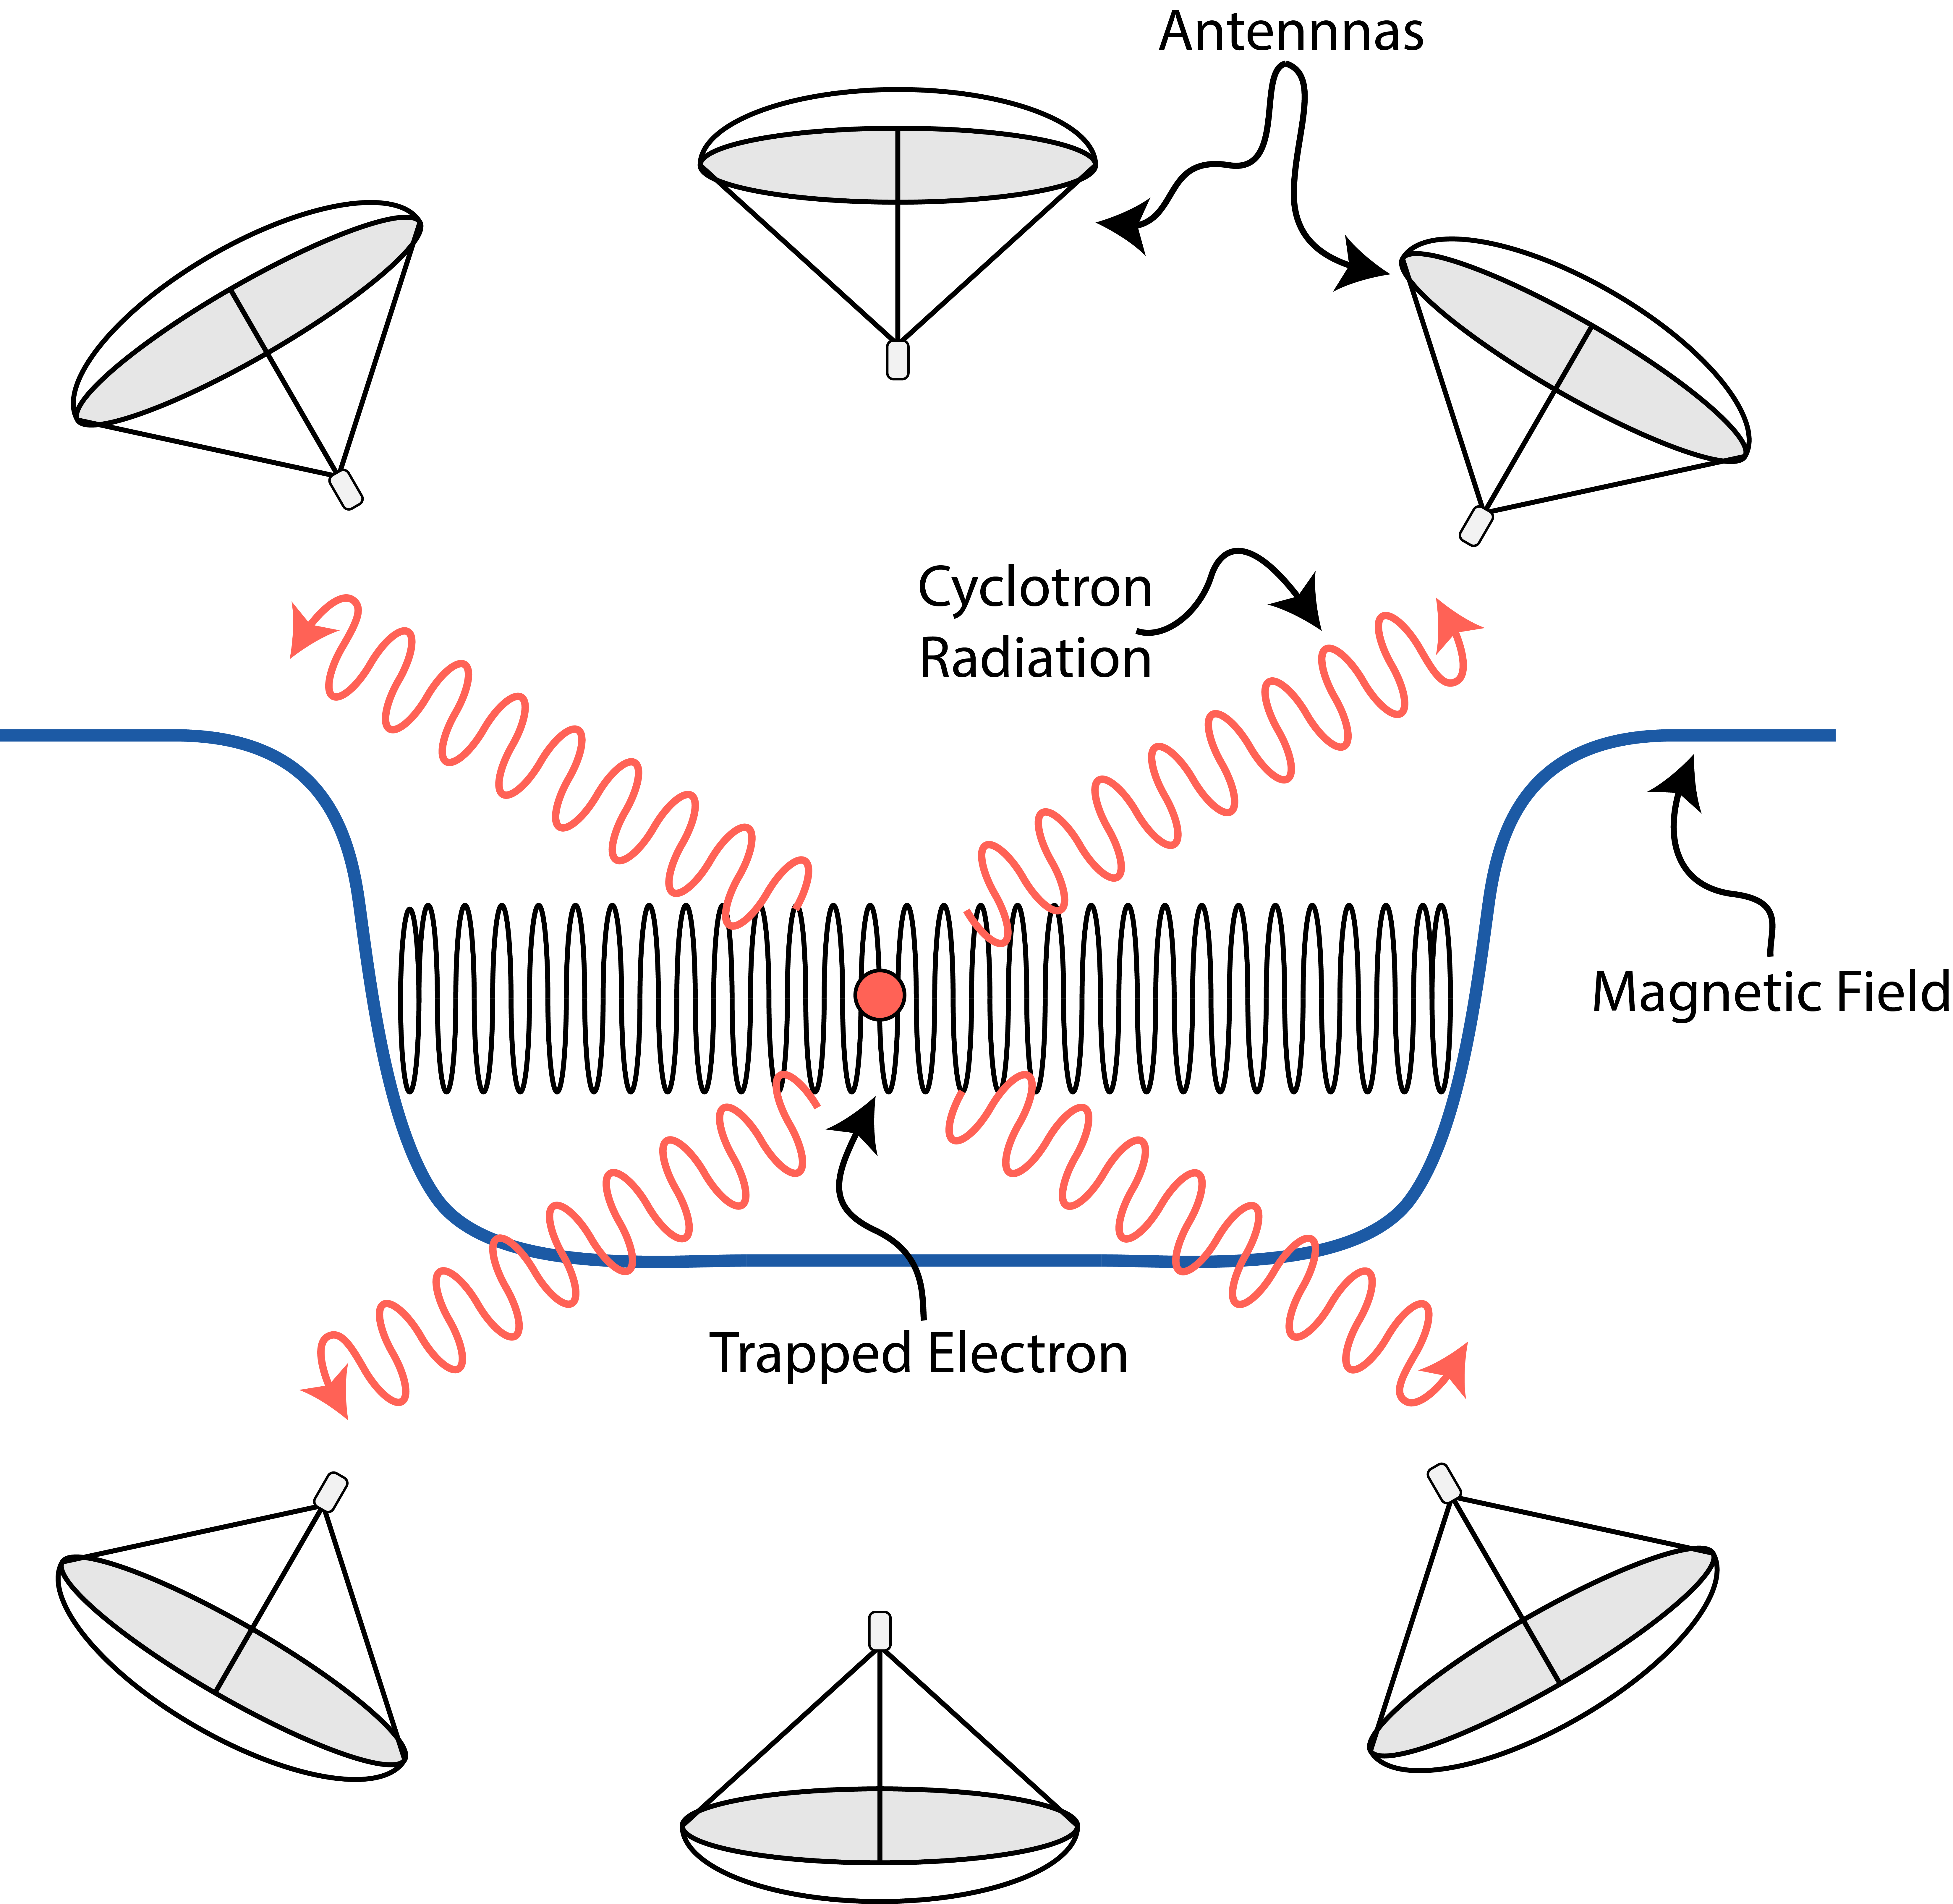
\includegraphics[width=0.5\textwidth]{figs/Chapter-3/230303_cres_cartoon.png}
    \caption{Caption}
    \label{fig:cres_cartoon}
\end{figure}

\subsection{Charged Particles in a Magnetic Trap}

\begin{figure}[htbp]
    \centering
    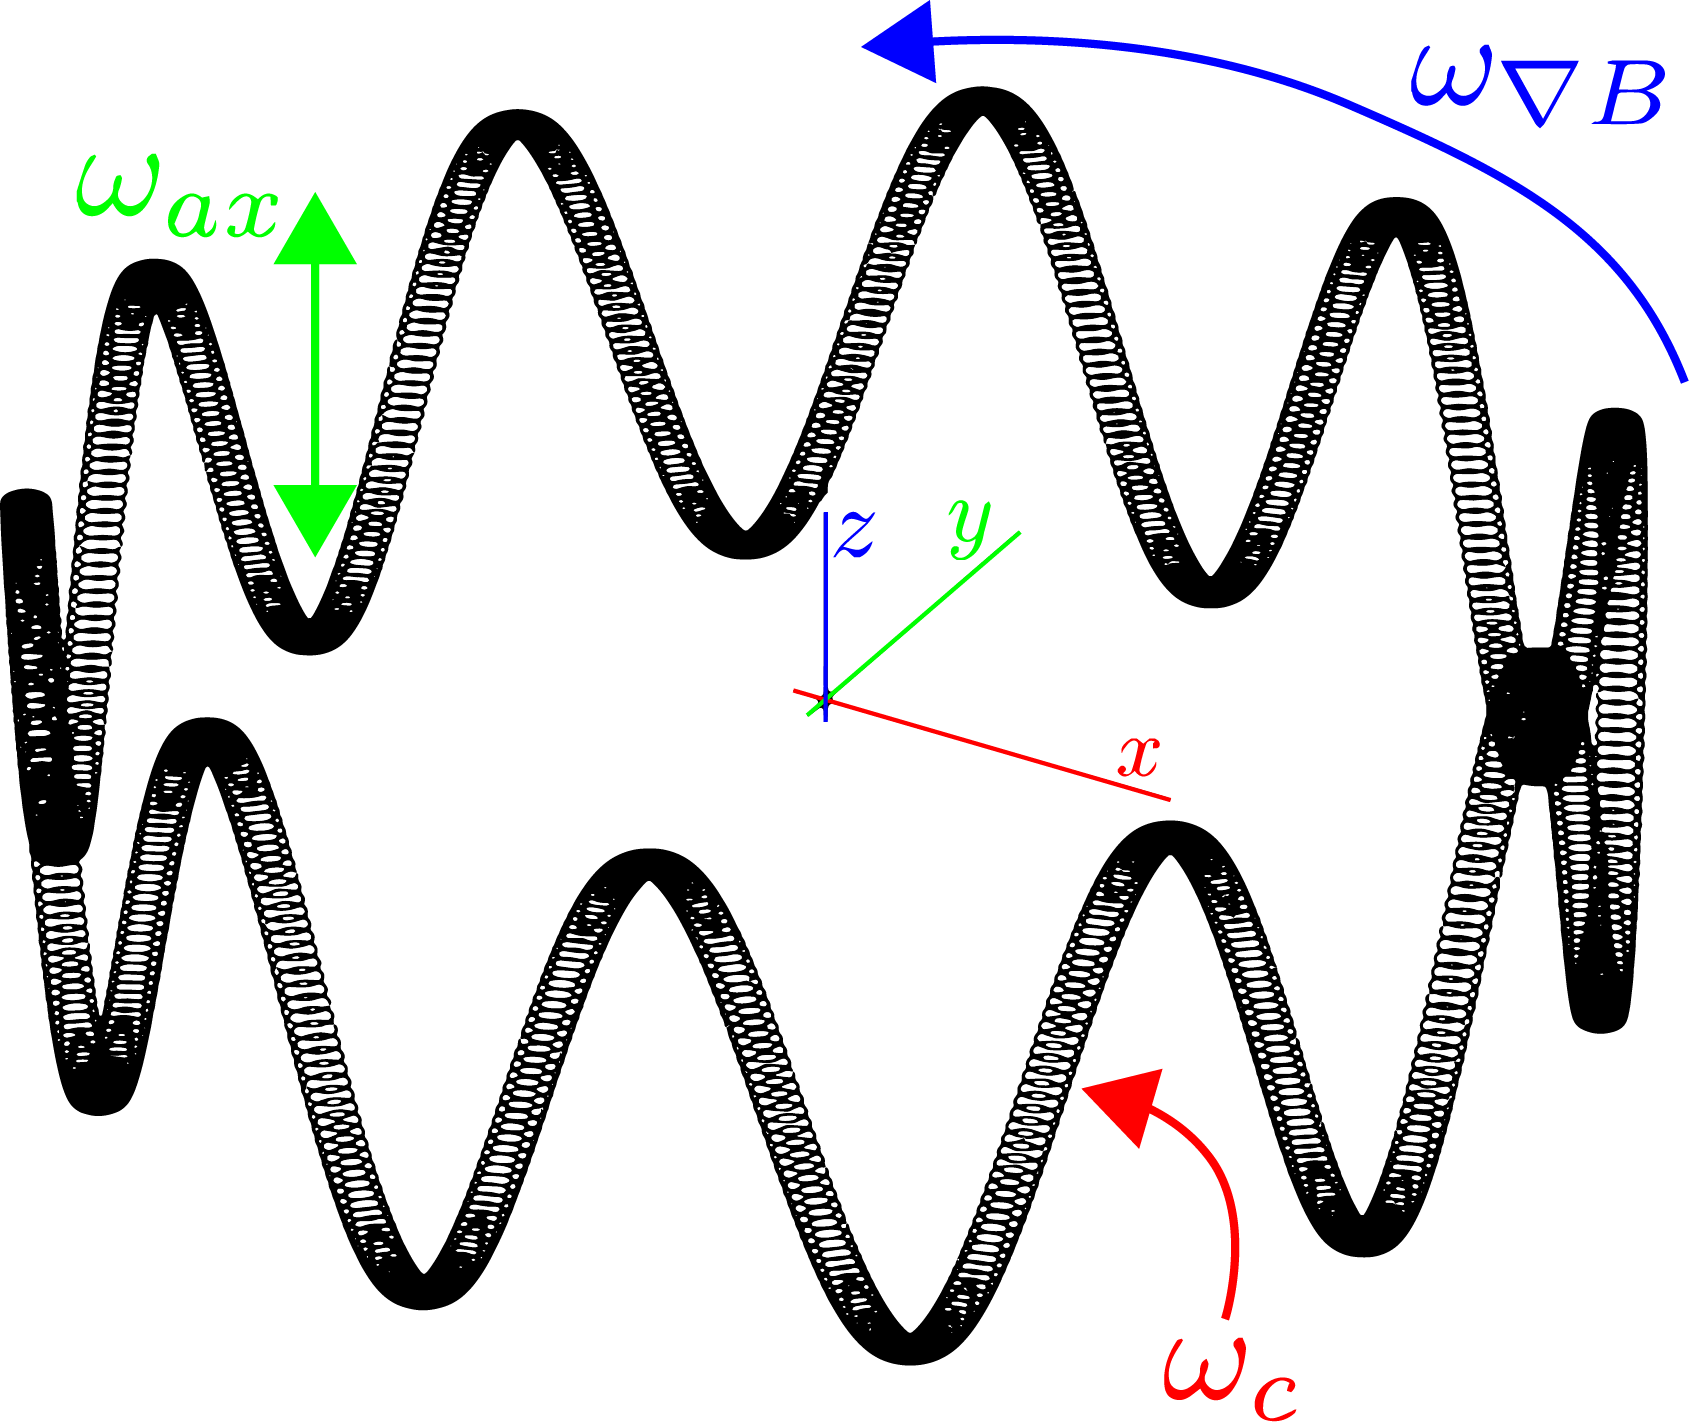
\includegraphics[width=0.5\textwidth]{figs/Chapter-3/230511_trapped_motion.png}
    \caption{Caption}
    \label{fig:chap3-trapped-electron-motion}
\end{figure}

\subsection{Radiation from a Charged Particle}

\section{The Project 8 Collaboration}

\subsection{Neutrino Mass Sensitivity Goals}

\subsection{Phased Development Plans}

\begin{figure}[htbp]
    \centering
    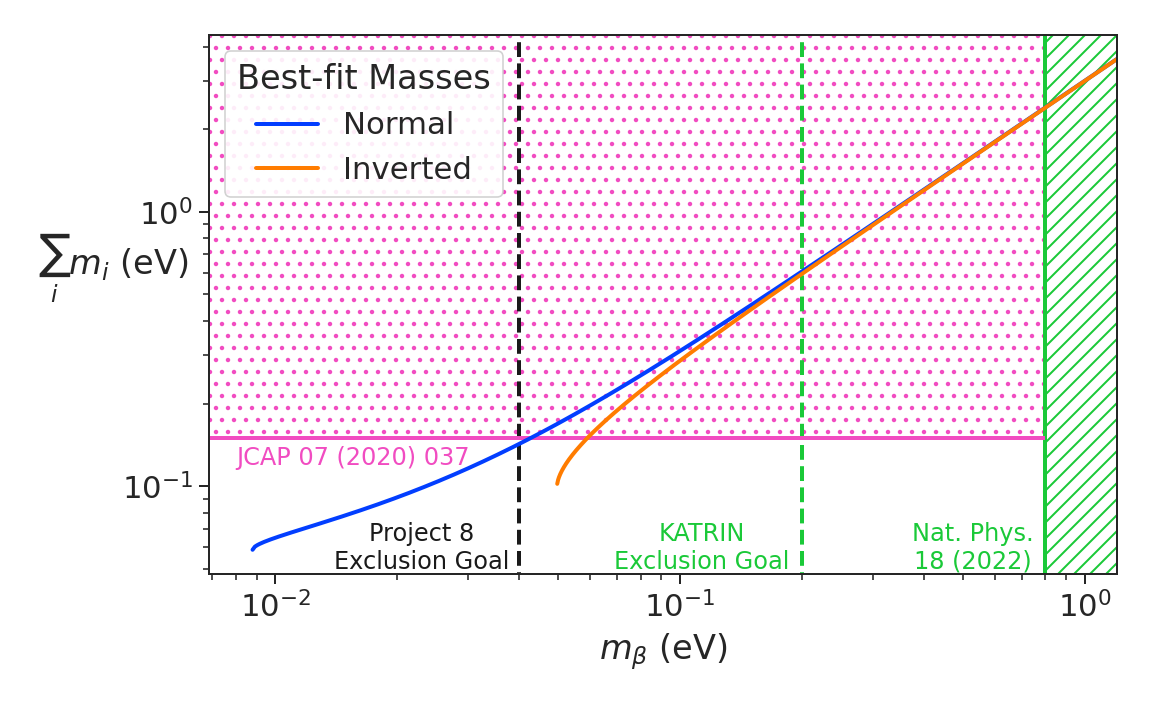
\includegraphics[width=0.7\textwidth]{figs/Chapter-3/230303_sum_nu_mass_vs_m_beta_with_exclusion_and_goal.png}
    \caption{Caption}
    \label{fig:p8_nu_mass_goal}
\end{figure}

\cleardoublepage


\section{Phase II: First Tritium Beta Decay Spectrum and Neutrino Mass Measurement with CRES}

In Phase II Project 8 demonstrate the first ever measurement of the tritium beta-decay spectrum endpoint using the CRES technique, which lead to the first neutrino mass measurement by the Project 8 collaboration. This milestone was made possible by many improvements in the CRES technique and more developed understanding of CRES systematics, which takes an important first step towards larger scale measurments of the tritium beta-decay spectrum with CRES. In this section, I shall briefly describe some the important elements of the Phase II experiment, with the goal of contextualizing the research and development efforts for Phases III and IV of Project 8. For more complete descriptions of the work that lead to Project 8's Phase II results please refer to the many Phase II papers produced by the collaboration.

\subsection{The Phase II CRES Apparatus}

\begin{figure}[htbp]
    \centering
    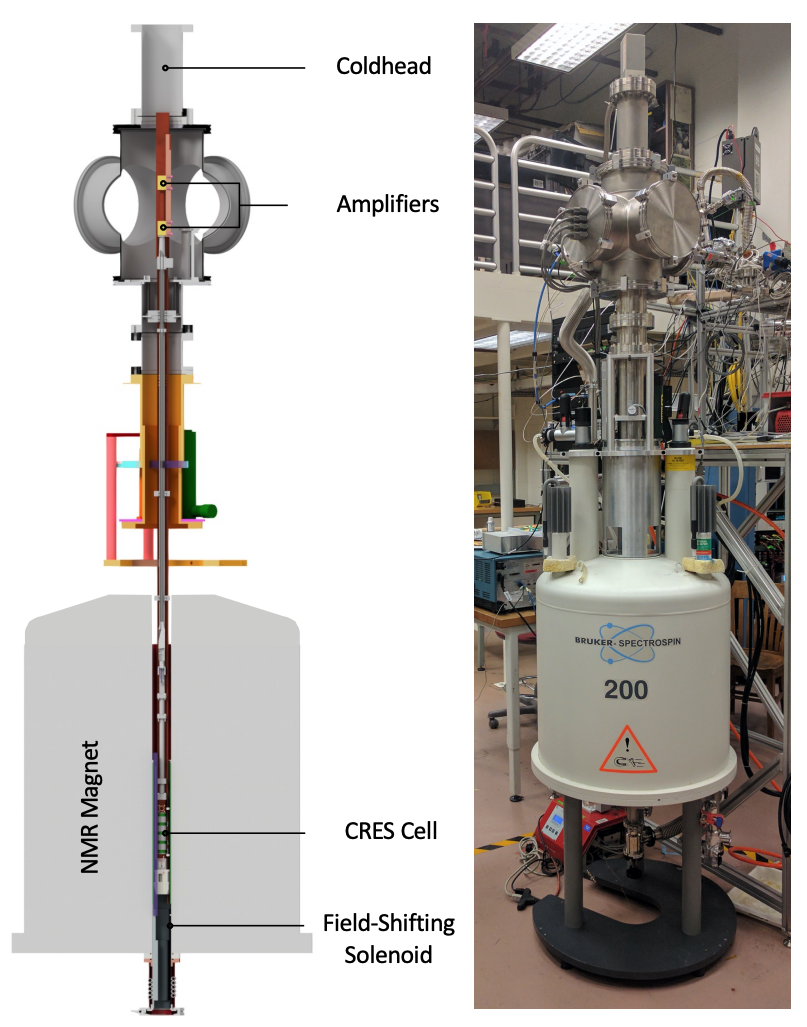
\includegraphics[width=0.55\textwidth]{figs/Chapter-3/phaseII_system.png}
    \caption{\label{fig:chap3-phase2-apparatus} The Phase II CRES apparatus used to perform the first measurement of the tritium beta-decay spectrum using CRES.}
\end{figure}

\subsubsection*{Magnet and Cryogenics}

The magnetic field for the the Phase II experiment is provided by a nuclear magnetic resonance (NMR) spectroscopy magnet with a central bore diameter of 52~mm (see Figure \ref{fig:chap3-phase2-apparatus}). The magnet produces a background magnetic field with an average value of 0.959~T and a 10~ppm variation across the bore diameter achieved using several shim coils built into the magnet. Using an external NMR field probe the variation of the magnetic field along the vertical axis of the magnet bore was measured to obtain an accurate model of the magnetic field so that the CRES cell could be positioned for optimal magnetic field uniformity.

An external solenoid magnet was installed inside the magnet bore to provide the ability to shift the magnitude of the background magnetic field by values on the order of a few mT. The solenoid has inside diameter of 46~mm and a length of 350~mm, which terminates in a vacuum flange that allows it to be inserted into the NMR magnet bore from the bottom. By shifting the value of the magnetic field by a few mT, the cyclotron frequencies of electrons produced by the 17.8~keV $^{83m}$Kr electron conversion line can be shifted over a range of frequencies on the order of 100~MHz. This allows one to study the frequency dependent behavior of multiple CRES systematics such as detection efficiency that directly affect the measured shape of the tritium spectrum. 

The inside of the magnet bore diameter was pumped down to a vacuum of less than 10~$\mu$torr using a turbomolecular pump, which allows for cryogenic cooling of the CRES cell and RF system. Cooling power was supplied to the Phase II apparatus using a cryopump with its coldhead mounted above the primary magnet and CRES cell. This arrangement allowed for sufficient cooling power to be delivered to the amplifiers to cool them to a temperature of $\approx 40$~K, while keeping the amplifiers far enough from the magnet so as not to be damaged by the large field strength. Thermal contact between the coldhead, amplifiers, RF system, and CRES cell is achieved using a copper bar that runs the full length of the apparatus. To prevent freeze-out of $^{83m}$Kr on the walls of the CRES cell a separate heater was installed to keep the CRES cell near a temperature of 85~K during the operation of the experiment.

\subsubsection*{CRES Cell}

Located in the most uniform region of the magnetic field is the CRES cell, which is the region of the apparatus where radioactive decays of $^{83m}Kr$ and $T_2$ emit electrons that can be trapped and measured using CRES (see Figure \ref{fig:chap3-cres-cell}).
\begin{figure}[htbp]
    \centering
    \includegraphics*[width=0.65\textwidth]{figs/Chapter-3/apparatus.pdf}
    \caption{\label{fig:chap3-cres-cell} Diagram of the CRES cell portion of the Phase II apparatus.}
\end{figure}
The CRES cell is manufactured from a segment of cylindrical waveguide designed to operate at K-band frequencies near 26~GHz. The diameter of the waveguide determines which resonant modes of the waveguide will couple to the electron and transmit its radiation to the amplifiers. For Phase II a waveguide diameter of 1~cm was selected, which allows electrons to couple to the $\mathrm{TE}_{11}$ and $\mathrm{TM}_{01}$ cylindrical waveguide modes. To reduce complexity in modeling and analyzing the CRES data, it is ideal to select a diameter that prevents electrons from coupling to higher-order waveguide modes beyond the fundamental TE and TM modes. 

Around the exterior of the cylindrical waveguide are several magnetic coils used to produce magnetic traps inside the CRES cell volume. Without a magnetic trap electrons produced from decays inside the CRES cell quickly impact the cell wall, which prevents a measurement of their cyclotron frequency using CRES. Each coil along the length of the waveguide produces a separate trap that is approximately harmonic in shape. By independently controlling the currents provided to each coil the traps could be configured to have equal values of the magnetic field at the trap bottom despite a variable background magnetic field from the NMR magnet. 

Two primary magnetic trap configurations were used during the Phase II experiment. The first was a shallow trap configuration used primarily for it's high energy resolution to study systematics using $^{83m}$Kr decays, and the second was a deeper trap that could trap a higher percentage of pitch angles. The trade-off with this trap is that the higher trapping efficiency comes at the cost of lower energy resolution due to the greater variation in pitch angle. The deep trap was the trap used to measure the tritium beta-decay spectrum in Phase II.

The source gases were delivered into the CRES cell through a gas port located near the top end of the cylindrical waveguide. To prevent the gases from escaping the cell, vacuum tight RF transparent windows are needed to contain the tritium and krypton source gas across a 1~atm pressure differential, while still transmitting the cyclotron radiation without distortion. The crystalline material, $\mathrm{CaF}_2$, which has a thermal expansion coefficient similar to that of copper, was used for this purpose in the CRES cell. Two windows, each 2.4~mm thick, were used to seal off the ends of the CRES cell. The thickness of 2.4~mm corresponds to half of a cyclotron wavelength when one accounts for the permittivity of $\mathrm{CaF}_2$.

\subsubsection*{RF System}

The RF system in the Phase II apparatus transferred the cyclotron radiation from the CRES cell to the receiver chain that begins at the top of the apparatus, and performed the down-conversion and digitization to obtain signals that could be analyzed to determine the cyclotron frequencies of electrons in the CRES cell (see Figure \ref{fig:chap3-phase2_rf_chain}).
\begin{figure}[htbp]
    \centering
    \includegraphics*[width=0.6\textwidth]{figs/Chapter-3/230620_phase2_rf_chain.png}
    \caption{\label{fig:chap3-phase2-rf-chain} Caption}
\end{figure}

\subsection{CRES Track and Event Reconstruction}

\begin{figure}[htbp]
    \centering
    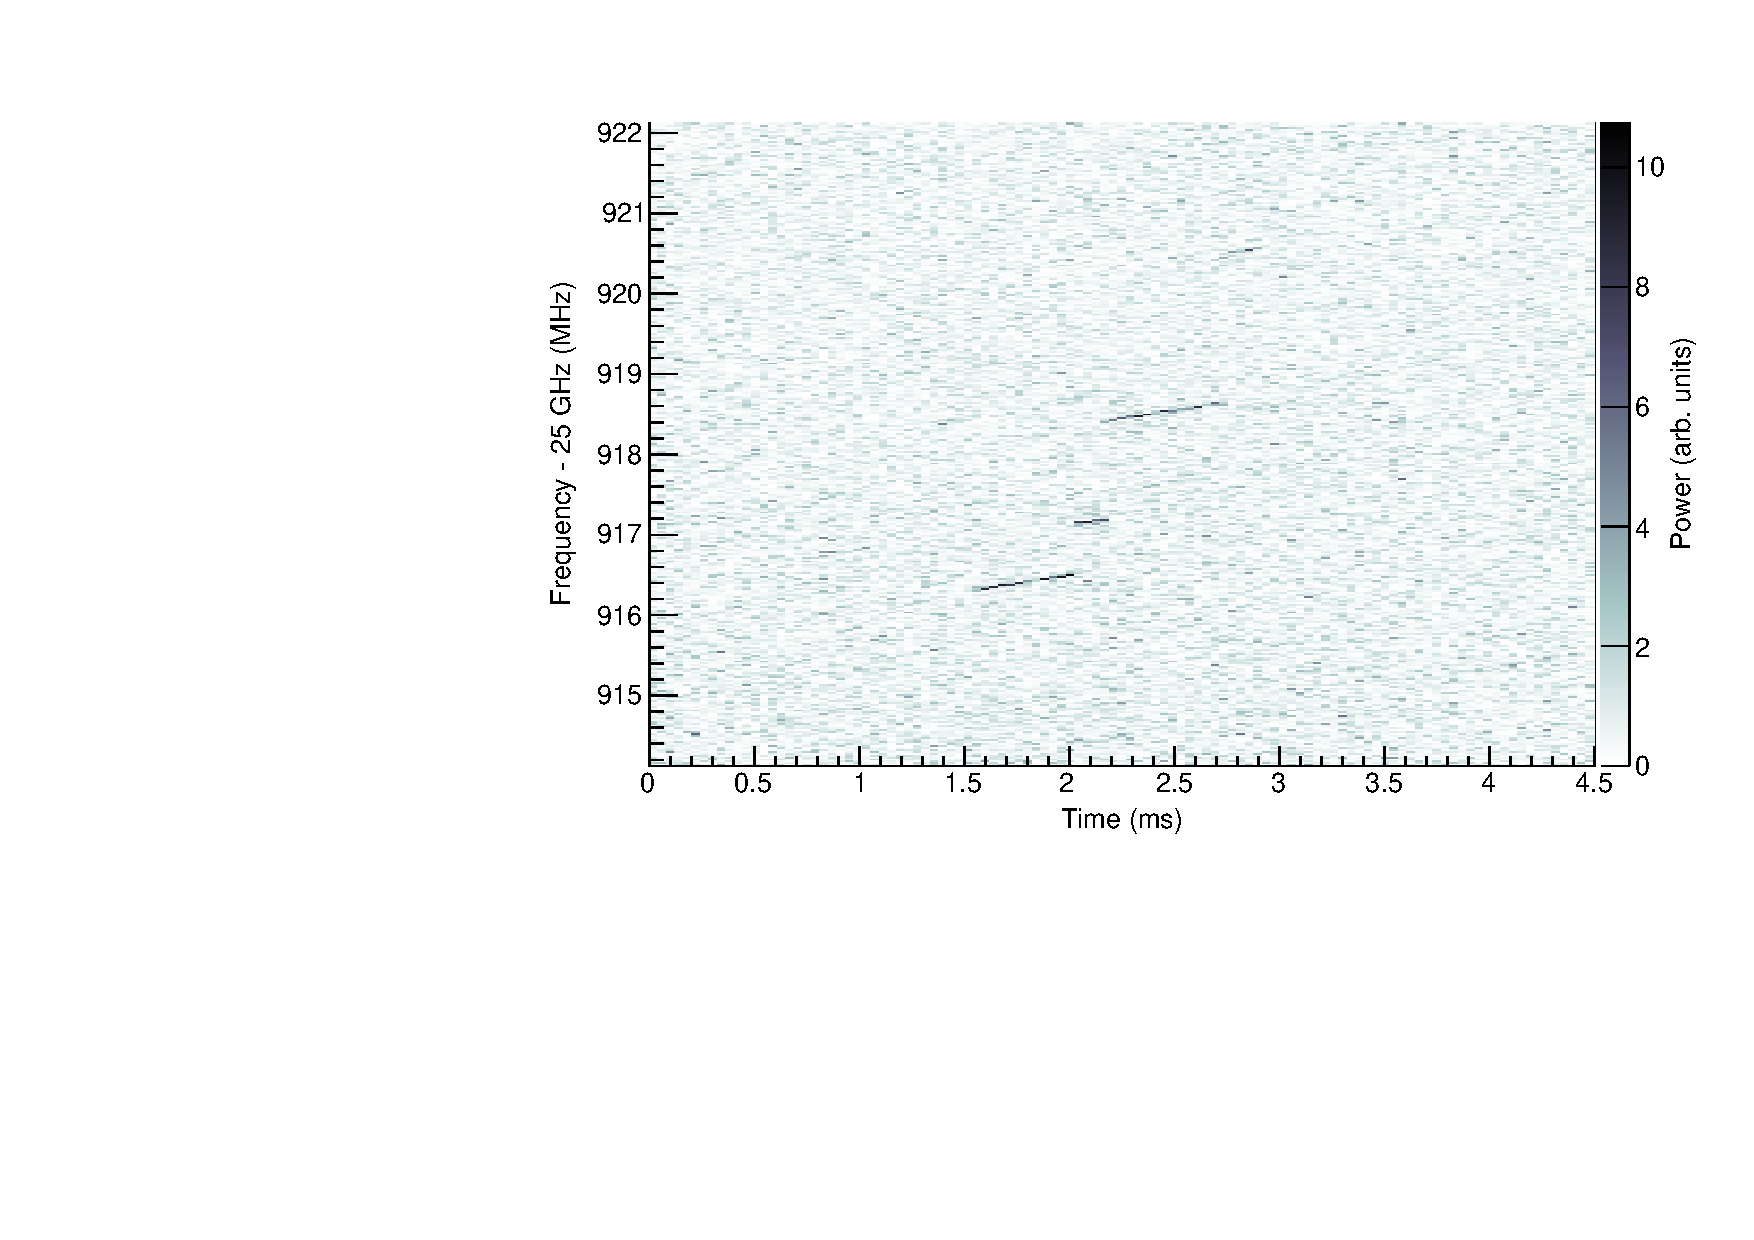
\includegraphics[width=0.7\textwidth]{figs/Chapter-3/T2_Event0.pdf}
    \caption{Caption}
    \label{fig:tritium_event0}
\end{figure}

\subsection{Measurements with Krypton}

\begin{figure}[htbp]
    \centering
    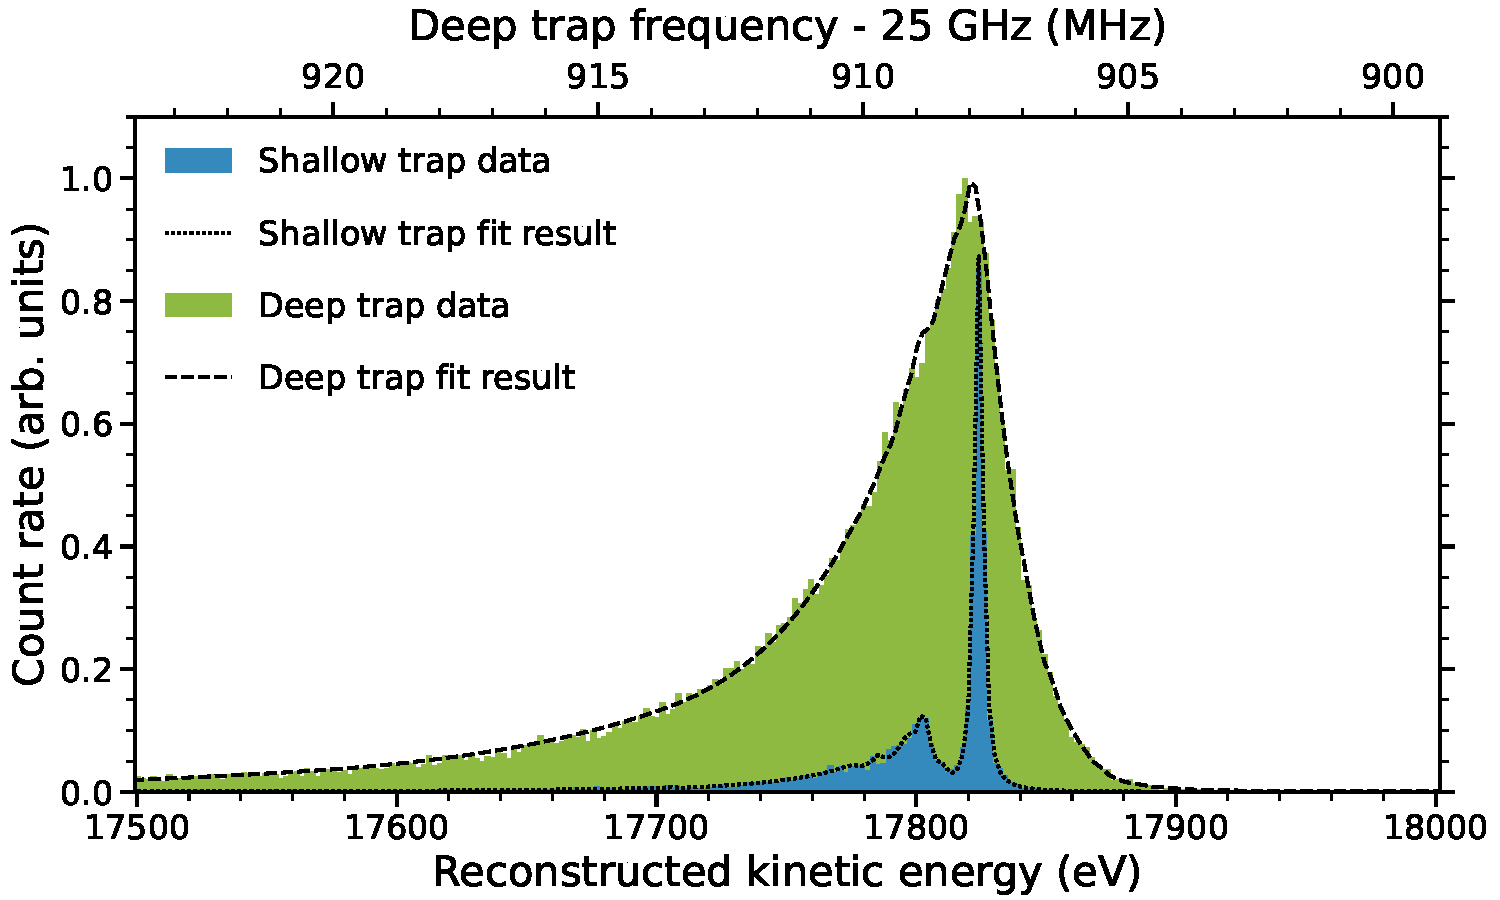
\includegraphics[width=0.7\textwidth]{figs/Chapter-3/kr_fit.pdf}
    \caption{Caption}
    \label{fig:krypton_fit}
\end{figure}

\begin{figure}[htbp]
    \centering
    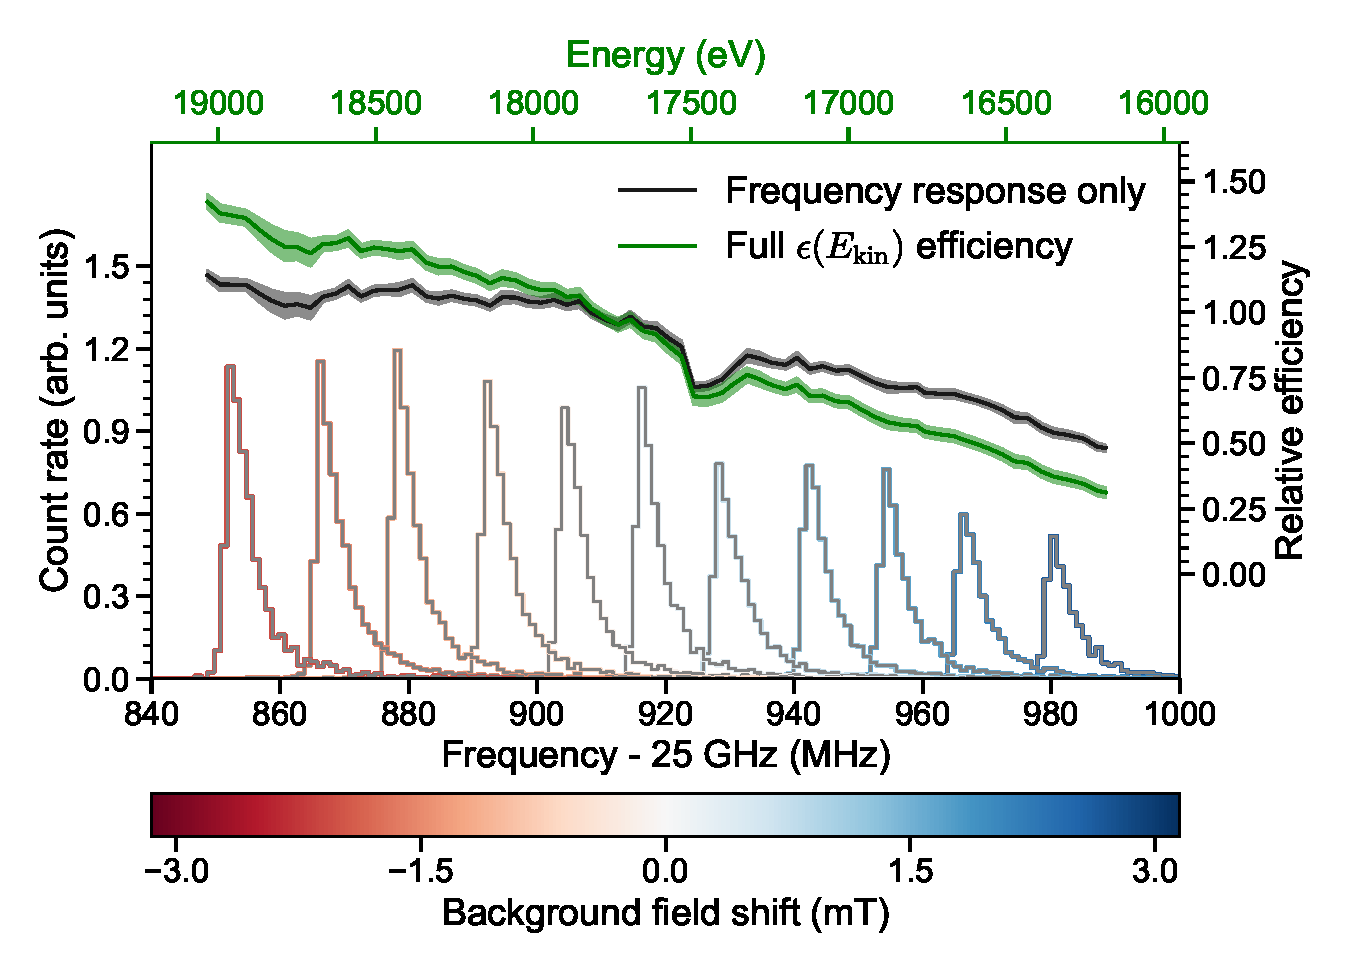
\includegraphics[width=0.7\textwidth]{figs/Chapter-3/fss_for_prl_plot.pdf}
    \caption{Caption}
    \label{fig:fss_plot}
\end{figure}

\subsection{Tritium Spectrum and Neutrino Mass Results}

\begin{figure}
    \centering
    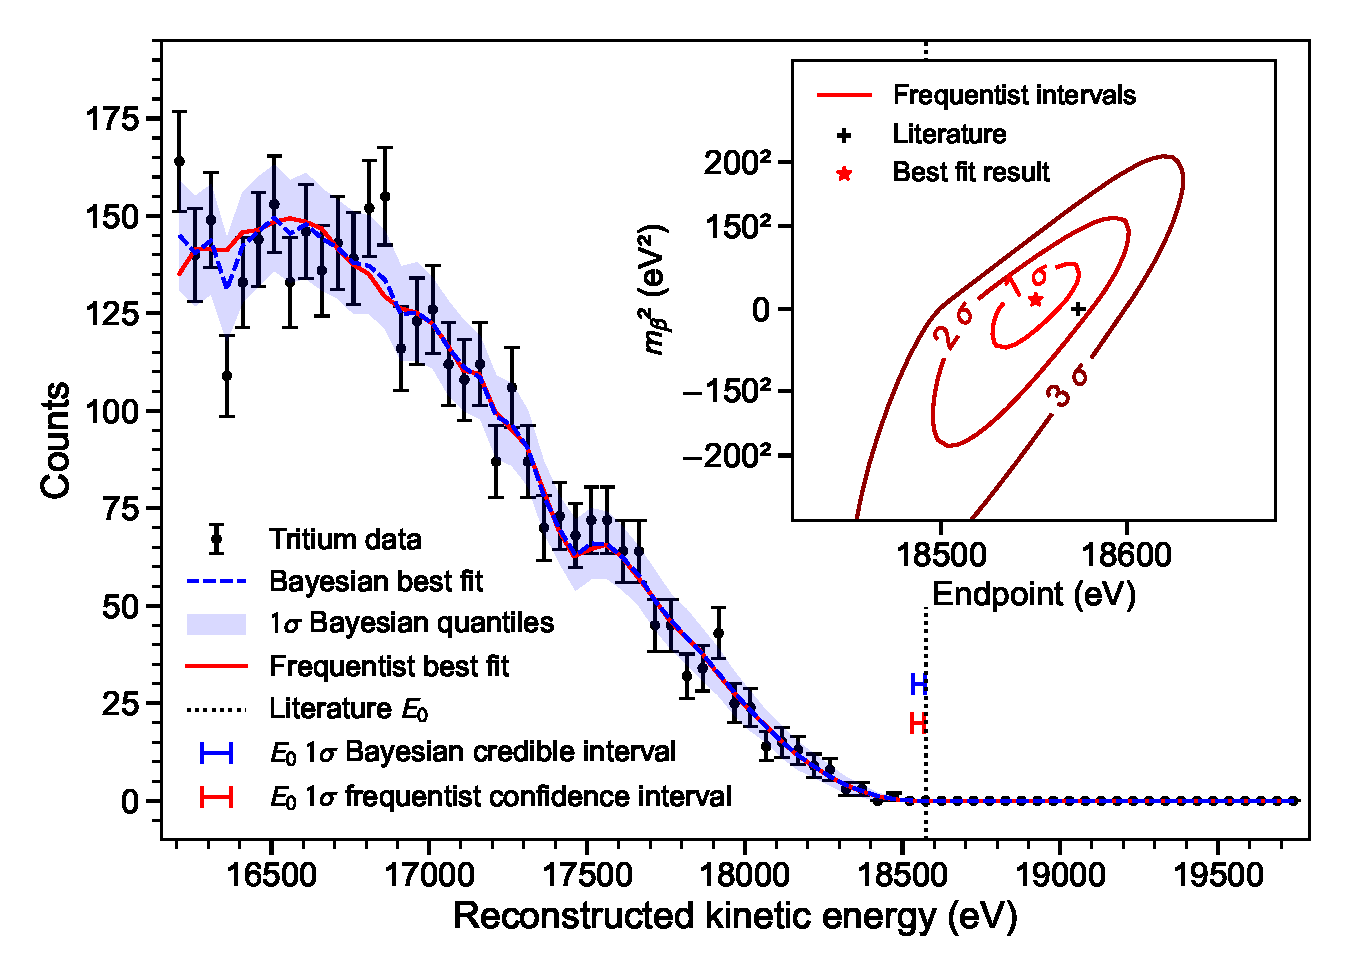
\includegraphics[width=0.7\textwidth]{figs/Chapter-3/12-03-22A_final_E0_real_data_phase_II_tritium_fit_1d.pdf}
    \caption{Caption}
    \label{fig:final_tritium_fit}
\end{figure}

\section{Phase III: Developing Free-space CRES Measurements with Antenna Arrays}

The goal of Phase III in the Project 8 experimental program is to develop the technologies and expertise required to build an experiment that uses CRES to measure the neutrino mass with a target sensitivity of 40~meV. One of the key technologies is a method for performing high resolution CRES measurements in a large volume, which allows one to observe a sufficient quantity of tritium to measure the low-activity endpoint region of the tritium spectrum. 

\subsection{The Basic Approach}

One possible approach, suggested in the original CRES publication, is to use many antennas to surround a volume of tritium gas in a magnetic field (see Figure \ref{fig:chap3-antenna-concept-cartoon}). When a decay occurs the electron will begin to emit cyclotron radiation that can be collected by the array and used to perform CRES.
\begin{figure}[htbp]
    \centering
    \includegraphics*[width=0.6\textwidth]{figs/Chapter-3/230614_antenna_cartoon.png}
    \caption{\label{fig:chap3-antenna-concept-cartoon}}
\end{figure}
Each antenna in the array collects only a small fraction of the electron's signal power, which is less than 1~fW for a 18.6~keV kinetic energy electron in a 1~T magnetic field. Scaling to large volumes with the antenna array approach is accomplished by increasing the number of antennas in the array, which increases the volume under observation proportionally, so that a sufficient population of tritium atoms can be observed to measure the tritium spectrum endpoint shape. 

Several features of the antenna array approach make it an attractive candidate technology for a large volume experiment. One example is the accurate position reconstruction made possible by the multichannel nature of the array. Using techniques like digital beamforming it is possible to estimate the radial and azimuthal positions of the electron in the magnetic trap with a precision significantly less than the size of the cyclotron wavelength. This capability allows one to perform event-by-event estimations of the magnetic field experienced by an electron, which is crucial to achieving high energy resolution with the CRES technique.

The easy availability of position information with the antennas array approach is potentially a unique advantage that provides significant flexibility in the magnetic field uniformity requirements compared to other proposed approaches to large volume CRES (see Chapter \ref{chap:cavity}). Spatial discrimination using digital beamforming leads to pileup reduction, which helps to reduce the potential of background events caused by missing tracks or by incorrectly clustering a group of tracks into an event. Limits on the background rate for a neutrino mass measurement with 40~meV sensitivity are stringent and the total activity of the tritium source for such an experiment is gigantic relative to the activity near the endpoint. Thus, pileup discrimination could be an important tool for a large scale CRES experiment.

Another beneficial quality of the antenna array approach is that the volume of the experiment can be scaled independent of frequency by simply adding more antennas to the array (see Figure \ref{fig:chap3-phaseiv-antenna}). Resonant cavities, the proposed alternative large volume CRES technology, are ideally operated in magnetic fields that cause electrons to move with cyclotron frequencies near the fundamental cavity resonance, to avoid complex coupling of the electron to many cavity modes simultaneously. This leads to a coupling between the cavity volume and the magnetic field magnitude, which forces one to lower the magnetic field in order to increase the experiment scale. Whereas, for antenna arrays, in principle there is no physical limitation on the size of the antenna array that can be used at a particular magnetic field. However, the nature of scaling an antenna array based experiment leads to rapidly increasing cost and complexity due to the large number of antennas, amplifiers, and data streams that require substantial computer processing power to effectively analyze.

\begin{figure}[htbp]
    \centering
    \includegraphics*[width=0.8\textwidth]{figs/Chapter-3/phaseiv_concept_sketch_ver2.png}
    \caption{\label{fig:chap3-phaseiv-antenna} A conceptual sketch of a large volume antenna array based CRES experiment to measure the neutrino mass.}
\end{figure}

\subsection{The FSCD: Free-space CRES Demonstrator}

The complex collection of new experimental techniques and methods that come together in the antenna array CRES technique require the construction of a small scale demonstration experiment designed to develop an understanding of the principles of antenna array CRES measurements and the relevant systematics. Without operating such an experiment it is not possible to develop a design for a large scale CRES experiment with sufficient confidence that the experiment is capable of measuring the shape of the tritium spectrum endpoint to the degree of accuracy required for 40~meV sensitivity to the neutrino mass. Therefore, Phase III of the Project 8 experimental program is primarily focused on the development and operation of demonstrator experiments to inform the design of the final Phase IV experiment.

Specifically for antenna array CRES, the associated demonstrator experiment in Phase III is called the Free-space CRES Demonstrator or FSCD. The goals of the FSCD include not only the development of antenna array CRES itself, but is also a capable neutrino mass measurement experiment in it's own right, with a target neutrino mass sensitivity of a few eV using a molecular tritium source.  

\subsubsection*{Magnetic Field}

The background magnetic field for the FSCD experiment is provided by a hospital-grade MRI magnet (see Figure \ref{fig:chap3-mri-magnet}). The magnet produces a magnetic field of approximately 0.958~T, which corresponds to a tritium spectrum endpoint frequency of approximately 25.86~GHz. 
\begin{figure}[htbp]
    \centering
    \includegraphics*[width=0.5\textwidth]{figs/Chapter-3/230614_mri_magnet.png}
    \caption{\label{fig:chap3-mri-magnet} An image of the MRI magnet installed in the Project 8 laboratory at the University of Washington, Seattle.}
\end{figure}
The magnet is installed in the Project 8 laboratory located at the University of Washington, Seattle, and is shimmed to produce a uniform magnetic field with variations on the ppm scale. Measurements of the magnetic field non-uniformities were performed using a NMR probe and rotational gantry to capture measurements of the magnetic field around an elliptical surface in the center of the MRI magnet. During the operation of the FSCD an array of Hall or NMR magnetometers could be used to periodical measure the magnetic field in order to quantify its time stability.

Inside the main magnetic field of the MRI magnet are additional magnets that provide the capability to shift the value of the background magnetic field as well as the magnets that produce the magnetic trap. Shifting the background value of the magnetic field on a scale of $O(\mu T)$ allows one to control the cyclotron frequencies of electrons with a fixed kinetic energy, which is key to effectively calibrating the FSCD. The preferred calibration method for the FSCD is a mono-energetic electron gun that can inject electrons into the magnetic trap with a known kinetic energy. In combination with the field shifting magnet one can vary the cyclotron frequencies of the electrons to measure the response of the antenna array as a function of the radiation frequency and electron position. This procedure not only characterizes the response of the antenna array but also provides further information on magnetic field uniformity, which important to achieving optimal energy resolution.

Several additional magnetic coils will need to included inside the MRI magnet to produce the magnetic trap. The ideal trap shape for CRES is the perfect magnetic box, which has a flat bottom and step function walls. Any variation in the average magnetic field experienced by an electron leads to changes in the cyclotron frequency that can make determining the true starting kinetic energy more difficult. This includes changes in the magnetic field caused by the walls of the magnetic trap as well as radial magnetic field variations. The perfect box trap is completely uniform and has infinitely steep walls that cause no change in the electron's cyclotron frequency as it is reflected from the trap wall, however, such a trap cannot be made from any combination of magnetic coils since it violates Maxwell's equations. The goal of magnetic trap design is to identify the configuration of coils that produces a trap that approximates the perfect box trap as closely as possible.

\subsubsection*{Antenna Array}

The canonical antenna array design for a CRES experiment is a uniform cylindrical array of antennas that surrounds the magnetic trap volume. Since the FSCD is a demonstrator experiment, the antenna array design is the simplest form of the uniform cylindrical array, which is a single circular ring of antennas with a diameter of 20~cm (see Figure \ref{fig:chap3-fscd-render}).
\begin{figure}[htbp]
    \centering
    \begin{subfigure}{0.5\textwidth}
        \includegraphics*[width=\textwidth]{figs/Chapter-3/230614_fscd_render.png}
        \caption{}
    \end{subfigure}
    \hfill
    \begin{subfigure}{0.4\textwidth}
        \includegraphics*[width=\textwidth]{figs/Chapter-3/230614_5slot_model.png}
        \caption{}
    \end{subfigure}
    \caption{\label{fig:chap3-fscd-render} (a) A model of the FSCD antenna array, magnetic trap, and tritium containment vessel design.(b) A more detailed model of a prototype design for the 5-slot waveguide antenna design.}
\end{figure}
Along this circle are sixty slotted waveguide antennas that fully populate the available space around the array circumference. In order to maximize the power collected from each electron it is optimal to cover as large a fraction of the solid angle around the magnetic trap as possible. 

The distance between antennas around the circumference of the array is proportional to the wavelength of the cyclotron radiation. Therefore, maximizing the solid angle coverage of the array, while minimizing channel count to keep the hardware and data acquisition costs manageable, biases one towards smaller array diameters. Antenna near-field effects limit the minimum diameter of the array for a given antenna design since the radiation from electron's that are too close to the array cannot be detected due to destructive interference caused by path-length differences from the electron to different points on the antenna surface. 

Slotted waveguide antennas are used in the FSCD antenna array due to their high efficiency and low loss, which comes from the lack of dielectric materials in the antenna structure. Coupling to the waveguide can be performed with a coaxial cable connected at the center or on either end of the waveguide. One of the drawbacks of waveguide antennas is the large amount of space required to fit them inside the limited MRI magnet volume. Alternative antenna designs, constructed from microstrip printed circuit boards require significantly less space at the cost of slightly higher energy loss in the antenna structure. 

The FSCD antenna design is a 5~cm long segment of WR-34 waveguide with 5 vertical slots cut into the side. The distance between slots along the length of the waveguide is a half wavelength for optimal power combination between the individual antenna slots. Each slot is offset from the center of the antenna face a small distance in order to most effectively couple the slot to waveguide modes inside the antenna.

The passive power combination achieved by placing 5 slots in a single waveguide is a compromise intended to reduce the cost and complexity of the antenna array system. Each additional channel in the array requires it's own cryogenic amplifier and also increase the required computer power to process the raw data collected by digitizing each channel. Passive summation, achieved by combining antennas into arrays axially, reduces the array channel count at the cost of losses from imperfect passive combination. Imperfect passive combination is caused by effects such as re-radiation of energy from and destructive interference between slots in the waveguide antenna. 

Interference and re-radiation eventually limit the achievable the axial extent of passive power combination. The 5-slot designed developed for the FSCD is optimized to minimize the impact of these losses while achieving the maximum amount of axial coverage with a single ring of antennas. Scaling beyond the volume covered by a single ring of antennas is achieved by stacking additional rings of antennas together to cover a larger trap volume for a higher statistics measurement of the tritium spectrum endpoint region. A likely scenario for the FSCD experiment involves a staged experiment approach, where first a series of measurements is performed using only a single ring of antennas followed by experiments that add additional rings to the FSCD. The goal would be to first understand the principles of antenna array CRES using the simplest possible experiment, before attempting to scale the technique by expanding the antenna array size. 

\subsubsection*{Tritium Source}

While the primary purpose of the FSCD is as a technology demonstrator, it is unlikely for the collaboration to gain the required confidence in the antenna array CRES technique to perform neutrino mass measurements at the 40~meV sensitivity level without an intermediate scale measurement of the neutrino mass using antenna array CRES. Therefore, the FSCD has an additional scientific goal of measuring the neutrino mass with a rough sensitivity goal of a few eV. This level of precision is achievable using a source of molecular tritium with a volume of approximately 1~L at a density comparable to potential Phase IV scenarios.

Unlike previous CRES experiments, where the tritium source could be co-located with the receiving antenna inside a waveguide transmission line, the tritium source in the FSCD is thermally isolated from the antenna array to avoid freeze-out of the tritium molecules. The tiny radiation power emitted by electrons requires a system noise temperature of $\approx 10$~K or less, in order to detect events at a high enough efficiency to reach the neutrino mass sensitivity goals of the experiment. Achieving a system noise of 10~K requires that the antenna array and amplifiers operate at cryogenic, liquid helium temperatures of $\approx 4$~K, which significantly lowers the vapor pressure of molecular tritium. By keeping the molecular tritium isolated in an RF-transparent vessel the tritium gas can be kept at a relatively warmer temperature in the range of 30~K to avoid the accumulation of tritium on the experiment surfaces. 

\subsubsection*{Data Acquisition and Reconstruction}

A fundamental change in the data acquisition system for the FSCD is the shift from single to multi-channel reconstruction. This transition results in a significant increase in the data-generation rate, which is linearly related to the number of independent channels in the array. The larger data volume coincides with an increased demand for computer processing power based on the need for more precise signal reconstruction algorithms driven by the FSCD and Phase IV sensitivity goals. Therefore, the data acquisition system for the FSCD is likely to represent a significantly larger fraction of the experiment cost and complexity than previous CRES experiments.

Each antenna in the array is connected to a cryogenic amplifier and down-converted from the 26~GHz CRES frequency using an IQ-mixer to reduce the size of the analysis window in which the tritium spectrum is measured. Using an LO with a frequency of approximately 25.80~GHz the antenna array signals can be digitized at a rate of 200~MHz, which is sufficient bandwidth to resolve the complete sideband spectrum produced by axial oscillations of electrons in the FSCD magnetic trap. 

Direct storage of the raw FSCD antenna array data is undesirable, since the estimated amount of raw data generated is $O(1)$~exabyte per year. The management and storage of such a large dataset is infeasible for a demonstrator experiment on the scale of the FSCD and would represent a large fraction of the budget for a Phase IV scale antenna array based CRES experiment. Therefore, a sub-goal of the FSCD experiment is the development of real-time reconstruction methods that could reduce the raw data volume by detecting and reconstructing CRES events in real-time. The ultimate goal would be a complete real-time reconstruction pipeline that takes raw voltages samples from the antenna array and returns estimates for the starting kinetic energies of CRES events in the data.

The feasibility of a real-time reconstruction pipeline rests on the development of computationally efficient algorithms that can be implemented without the need for enormous computing resources. One challenge with the antenna array approach is that the small radiation power of a single electron is distributed between each channel in the array, such that reconstruction using only the information in a single channel is not possible. Therefore, the simply performing the initial step in reconstruction --- signal detection --- requires orders of magnitude more computational power than previous CRES experiments. This operation will then be followed by other, potentially more expensive, reconstruction steps that are required in order to determine the kinetic energy of the electron.

